\section{Results}
\label{sec:results}

\subsection{PrexSyn achieves state-of-the-art accuracy and speed in chemical space projection}
\label{sec:results:projection}


We first evaluate PrexSyn on the chemical space projection task.
This task involves finding synthesizable analogs for given molecular graphs.
Two benchmark datasets with different emphases \citep{luo2024projecting,gao2025generative} are used for evaluation: 
(1) \textbf{Enamine testset}: 1,000 molecules curated from the Enamine REAL database \citep{shivanyuk2007enamine}, used to assess how well the model covers the synthesizable chemical space.
(2) \textbf{ChEMBL testset}: 1,000 molecules from ChEMBL \citep{gaulton2012chembl}, which are not necessarily synthesizable with the Enamine building blocks and reactions, used to test the model's ability to find synthesizable analogs for arbitrary molecular graphs.

To run the projection task, we first compute the ECFP4 fingerprint of each molecule in the testset and embed it into prompt vectors, which condition the model to generate postfix notations of synthesis.
64, 128, and 256 independent samples are drawn for each target molecule. The product with the highest fingerprint similarity to the input molecule is selected as the projection result in accordance with the evaluation procedure of previous studies.
All inference is conducted on a single NVIDIA 4090 GPU.

As shown in Table \ref{tab:projection} and Figure \ref{fig:projection}, PrexSyn significantly surpasses previous methods on both datasets in terms of quality and efficiency.
In particular, it achieves a record-high reconstruction rate of 94.06\% on the Enamine testset, along with a Tanimoto similarity score over Morgan fingerprints of 0.9859, whereas the previous best model only achieves a reconstruction rate of 76.8\% and a similarity score of 0.95. 
This result shows that PrexSyn nearly perfectly covers the synthesizable chemical space defined by the Enamine building blocks and reactions, thereby establishing a strong foundation for more complex chemical space exploration tasks.
On the ChEMBL testset, PrexSyn achieves a reconstruction rate of 28.32\% and a similarity score of 0.7533, setting a new state-of-the-art performance, which demonstrates its strong capability to find similar analogs for molecules beyond the defined chemical space.

In addition to the improved accuracy, PrexSyn is substantially faster, taking an average of only 0.10 seconds per target with a sample size of 64 and 0.26 seconds with a sample size of 256, which is at least 60 times faster than the highest-accuracy baseline.
The high inference speed of PrexSyn is enabled by two factors: the C\texttt{++}-based detokenizer (Section~\ref{sec:method:data}) and the stronger model capacity that eliminates the need for inference-time search.
While previous methods \citep{luo2024projecting,gao2025generative,lee2025rethinking} rely on beam search or other inference-time scaling techniques to maximize the similarity scores, PrexSyn simply generates multiple postfix notations independently in parallel and convert all of them into synthetic pathways at once.
This efficiency makes PrexSyn practical for large-scale applications.

We also trained variants of PrexSyn with different amounts of training data to evaluate the effect of data volume on model performance.
As shown in Figure \ref{fig:projection}c, the reconstruction rate consistently increases as the training data scale grows, highlighting the benefit of large-scale training.
Notably, training the full-scale PrexSyn on 1.3 billion samples requires only 48 hours on 2 NVIDIA H100 GPUs.
This training cost is substantially lower than that of SynFormer \citep{gao2025generative} and ReaSyn \citep{lee2025rethinking}.
For comparison, SynFormer required 6 days on 8 A100 GPUs to train on 742 million samples, and ReaSyn required 5 days on 16 A100 GPUs to train on 512 million samples. 


\begin{table*}[tb]
  \small
  \caption{Chemical space projection results. \textit{Recons.\%} denotes the reconstruction rate, defined as the fraction of molecules with a similarity score of 1. \textit{Similarity} denotes the Tanimoto similarity based on ECFP4 (Morgan) fingerprint. PrexSyn achieves both the highest accuracy and the highest efficiency.}
  \label{tab:projection}
  \centering
  \begin{adjustbox}{max width=1\textwidth}
  \begin{tabular}{l cc cc c}
\toprule
 & \multicolumn{2}{c}{Enamine REAL} & \multicolumn{2}{c}{ChEMBL} \\
Method & Recons.\% & Similarity & Recons.\% & Similarity & Time/Target \\
\midrule
SynNet \citep{gao2021amortized} & 11.0\% & 0.57 & \phantom{0}5.4\% & 0.43 & - \\
ChemProjector \citep{luo2024projecting} & 46.0\% & 0.81 & 13.0\% & 0.60 & 5.15s$\pm$4.58s \\
SynthesisNet \citep{sun2024procedural} & - & - & \phantom{0}9.2\% & 0.53 & - \\
% \addlinespace[0.3em]
SynLlama \citep{sun2025synllama} & 69.1\% & 0.92 & 19.7\% & 0.68 & 24.88s$\pm$13.24s \\
\addlinespace[0.3em]
SynFormer \citep{gao2025generative} & \makecell{66.10\%\\$\pm$0.65\%} & \makecell{0.9137\\$\pm$.0014} & \makecell{20.67\%\\$\pm$0.72\%} & \makecell{0.6737\\$\pm$.0005} & 3.45s$\pm$3.60s \\
\addlinespace[0.3em]
ReaSyn \citep{lee2025rethinking} & \makecell{74.93\%\\$\pm$0.17\%} & \makecell{0.9403\\$\pm$.0010} & \makecell{22.07\%\\$\pm$0.21\%} & \makecell{0.6740\\$\pm$.0007} & 19.71s$\pm$6.68s \\
\midrule
PrexSyn (\#samples=64) & \makecell{92.64\%\\$\pm$0.30\%} & \makecell{0.9819\\$\pm$.0005} & \makecell{25.40\%\\$\pm$0.31\%} & \makecell{0.7300\\$\pm$.0008} & {\bf 0.10s}$\pm$0.03s \\
\addlinespace[0.3em]
PrexSyn (\#samples=128) & \makecell{93.60\%\\$\pm$0.23\%} & \makecell{0.9845\\$\pm$.0004} & \makecell{27.18\%\\$\pm$0.33\%} & \makecell{0.7429\\$\pm$.0006} & 0.15s$\pm$0.04s \\
\addlinespace[0.3em]
PrexSyn (\#samples=256) & \makecell{\bf 94.06\%\\$\pm$0.26\%} & \makecell{\bf 0.9859\\$\pm$.0007} & \makecell{\bf 28.32\%\\$\pm$0.20\%} & \makecell{\bf 0.7533\\$\pm$.0011} & 0.26s$\pm$0.06s \\
\bottomrule
\end{tabular}

  \end{adjustbox}
\end{table*}

\begin{figure}[t]
  \centering
  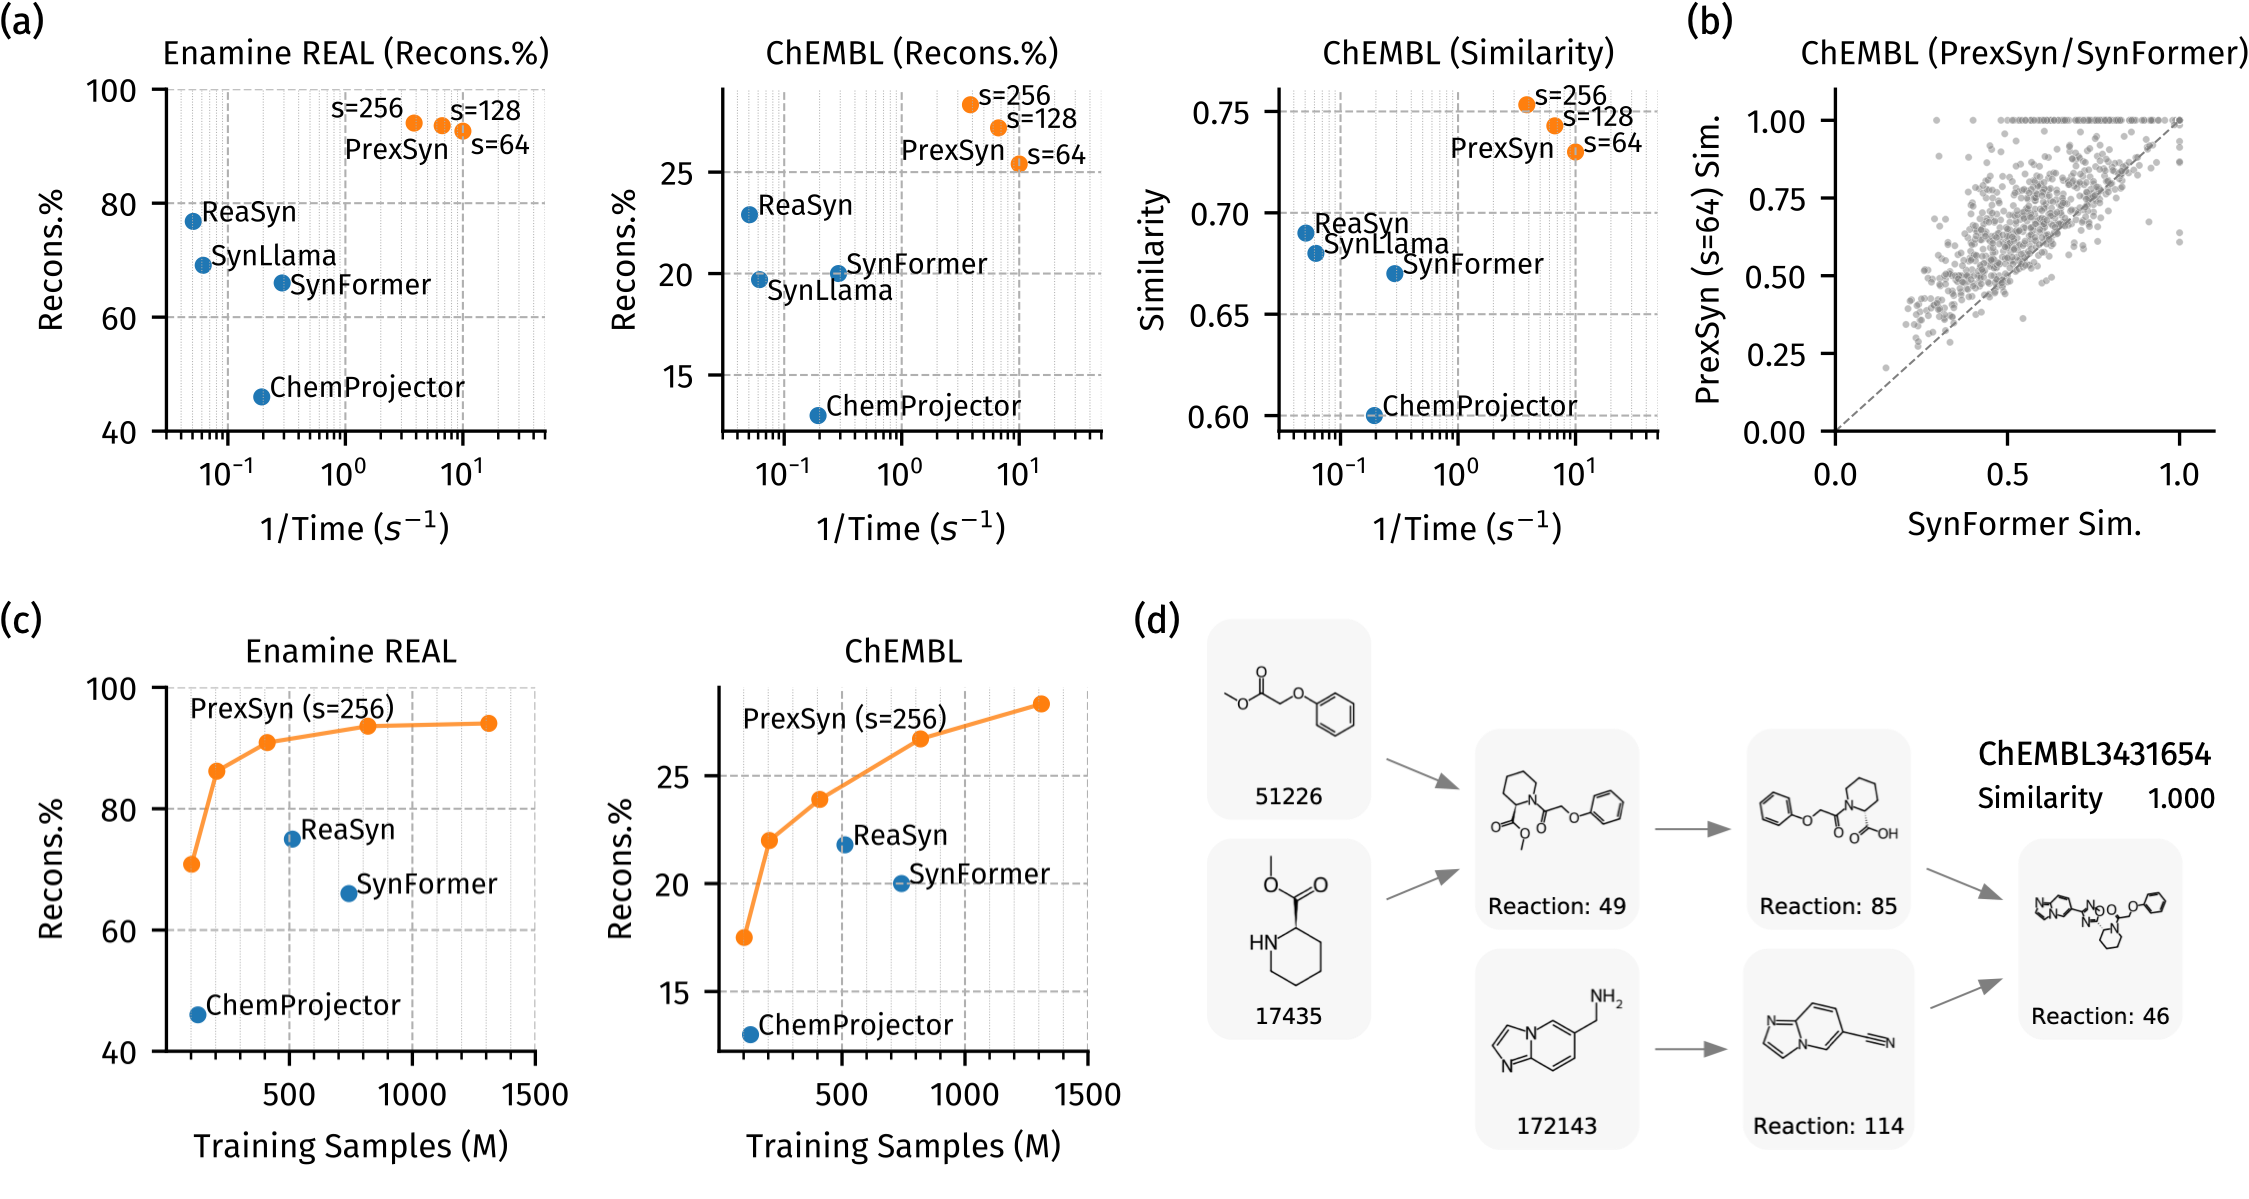
\includegraphics[width=\linewidth]{figures/fig2.png}
  \captionof{figure}{
    \textbf{(a)} Reconstruction rate/similarity versus inverse inference time on the Enamine and ChEMBL test sets. PrexSyn outperforms all baselines in both accuracy and efficiency.
    \textbf{(b)} Similarity of molecules projected by PrexSyn versus SynFormer on the ChEMBL test set. Each point corresponds to a molecule; points above the diagonal indicate higher similarity achieved by PrexSyn. The majority of points lie above the line, demonstrating consistently better performance.
    \textbf{(c)} Reconstruction rate versus training data scale. The reconstruction rate increases with larger training data, highlighting the benefit of large-scale training.
    \textbf{(d)} Example projection of a molecule from the ChEMBL test set that PrexSyn reconstructs perfectly. Tanimoto similarity using Morgan fingerprints is shown.
  }
  \label{fig:projection}
\end{figure}



\subsection{PrexSyn achieves state-of-the-art efficiency in synthesizable molecular sampling}
\label{sec:results:sampling}

% \paragraph{GuacaMol Benchmark}
To quantify the general sampling efficiency of PrexSyn, we conduct evaluation on seven multiproperty objectives and one rediscovery task from the GuacaMol benchmark suite \citep{brown2019guacamol}.
In these settings, scoring functions are treated as black boxes, which means no information about their internal form is visible to the model --- only the final scores are provided.
We set the initialization query of the $\mQ_0$ to Lipinski's Rule of 5 to generate drug-like molecules as starting candidates.
The optimizable term $\mC^\text{(opt)}$ is defined as the ECFP4 fingerprint and no constraint term is applied, $\mC^\text{(cstr)} = \varnothing$. Genetic algorithm is used to optimize the fingerprint $\mC^\text{(opt)}$ in alignment with previous methods \citep{gao2025generative,jensen2019graph,lee2025rethinking}.
The population size is set to 500, and at each iteration, 50 parents are sampled to generate 50 offspring through crossover.

We compare PrexSyn with both synthesis-agnostic and synthesis-based baselines.
All methods are given a budget of 10,000 oracle calls, and AUC-Top10 scores are reported following previous studies \citep{gao2022sample}.
As shown in Table \ref{tab:optim_guacamol}, PrexSyn achieves the highest average score on 6 out of 8 tasks, outperforming all synthesis-agnostic and synthesis-based baselines.

These results highlight the advantage of the query-space optimization paradigm enabled by PrexSyn.
We attribute the high sampling efficiency of PrexSyn to two main factors:
First, the high coverage of synthesizable chemical space of PrexSyn provides access to a much larger and more diverse set of feasible molecules, which increases the likelihood of finding high-scoring candidates.


Second, the property-based queries are numerical and therefore provide a well-structured optimization landscape that is easier to navigate.
Moreover, even when a query does not correspond to any valid molecule, the model can still generate molecules that approximate the desired properties, thereby smoothing the optimization landscape.
This is in contrast to the discrete and sparse search spaces of synthetic trees, where the action space of building block selection is intractably large and valid pathways are sparse because not all combinations of building blocks and reaction templates are valid.

As shown in Figure~\ref{fig:optimization}a, PrexSyn successfully reconstructs the target molecule and discovers multiple high-scoring analogs in the Celecoxib Rediscovery benchmark, whereas methods that directly search over synthetic trees fail to do so: SynFlowNet reports top 10 average similarity of 0.48 \citep{cretu2024synflownet}, and SyntheMol achieves an AUC-Top10 of only 0.527 (Table~\ref{tab:optim_guacamol}).




\begin{table*}[tb]
  \small
  \caption{
    GuacaMol benchmark results measured by AUC-Top10 \citep{gao2022sample}.
    DoG-Gen \citep{bradshaw2020barking} generates synthetic pathways but does not guarantee the validity of building blocks; therefore, its synthesizability is marked as neither yes nor no (\ding{117}).
    PrexSyn achieves the highest sampling efficiency on 6 out of 8 targets while maintaining synthesizability.
  }
  \label{tab:optim_guacamol}
  \centering
  \begin{adjustbox}{max width=1\textwidth}
  \begin{tabular}{l c cccccccc}
\toprule
Method & Syn. & Amlo. & Fexo. & Osim. & Peri. & Rano. & Sita. & Zale. & Cele.\\
\midrule
REINVENT \citep{olivecrona2017molecular} & \xmark & 0.635 & 0.784 & 0.837 & 0.537 & 0.760 & 0.021 & 0.358 & 0.713 \\
GraphGA \citep{jensen2019graph} & \xmark & 0.651 & 0.785 & 0.829 & 0.533 & 0.745 & 0.524 & 0.458 & 0.682 \\
MolGA \citep{tripp2023genetic} & \xmark & 0.688 & 0.825 & 0.844 & 0.547 & 0.804 & \bf 0.582 & 0.519 & 0.567 \\
\midrule
DoG-Gen \citep{bradshaw2020barking} & \ding{117} & 0.537 & 0.697 & 0.776 & 0.475 & 0.712 & 0.048 & 0.123 & 0.466 \\
SynNet \citep{gao2021amortized} & \cmark & 0.567 & 0.764 & 0.797 & 0.559 & 0.743 & 0.026 & 0.341 & 0.443 \\
SyntheMol \citep{swanson2024synthemol} & \cmark & 0.004 & 0.703 & 0.823 & 0.013 & 0.767 & 0.000 & 0.000 & 0.527 \\
SynthesisNet \citep{sun2024procedural} & \cmark & 0.608 & 0.791 & 0.810 & 0.524 & 0.741 & 0.313 & \bf 0.528 & 0.582 \\
SynFormer \citep{gao2025generative} & \cmark & 0.696 & 0.786 & 0.816 & 0.530 & 0.751 & 0.338 & 0.478 & 0.559 \\
ReaSyn \citep{lee2025rethinking} & \cmark & 0.678 & 0.788 & 0.820 & 0.560 & 0.742 & 0.342 & 0.492 & 0.754 \\
\midrule
PrexSyn & \cmark & \makecell{\bf 0.781\\$\pm$.023} & \makecell{\bf 0.837\\$\pm$.013} & \makecell{\bf 0.855\\$\pm$.007} & \makecell{\bf 0.714\\$\pm$.010} & \makecell{\bf 0.807\\$\pm$.009} & \makecell{0.471\\$\pm$.030} & \makecell{0.504\\$\pm$.018} & \makecell{\bf 0.801\\$\pm$.005} \\
\bottomrule
\end{tabular}

  \end{adjustbox}
\end{table*}



\subsection{PrexSyn enables molecular generation with composite property queries}

We next design three query tasks that simulate real-world drug discovery scenarios where composite property constraints are involved, as summarized in Table \ref{tab:query}.
For each task, we generate 1,000 postfix notations and score the product molecules according to how well they satisfy the specified query.
We report the mean and standard deviation of both the average score and the diversity of the top 5\% and top 10\% highest-scoring molecules across 5 independent runs.
Diversity is quantified as 1 minus the average pairwise Tanimoto similarity between Morgan fingerprints of the generated molecules \citep{jin2020multi}.

\paragraph{Task 1} evaluates the generation of drug-like molecules that satisfy Lipinski's Rule of Five \citep{lipinski2004lead,chagas2018drug}, expressed as a conjunction of multiple property constraints.
Molecules are scored between 0 and 1 according to the fraction of conditions satisfied.
The generated set achieves an average score of 0.9549, with the top 5\% and 10\% of molecules achieving perfect scores of 1.0000.
These top samples also maintain high diversity (above 0.89), indicating that the model produces a broad and varied set of Lipinski-compliant molecules.

\paragraph{Task 2} is inspired by the GuacaMol benchmarks \citep{brown2019guacamol}, which involve finding analogs of existing drugs with modified physicochemical properties.
Unlike the original GuacaMol benchmark, this task treats objectives as whitebox desiderata rather than blackbox oracles. 
Generated molecules are evaluated using the corresponding GuacaMol scoring functions, ranging from 0 to 1, with higher scores indicating better satisfaction of the desired properties.
On the Cobimetinib optimization benchmark (Task 2), our best molecule achieves a score of 0.9326, with the top 5\% and 10\% averaging 0.8975 and 0.8848, respectively.
For comparison, a graph-based approach that explicitly optimizes the four conditions, rather than treating the scoring function as a black box, reported a top score of 0.93 \citep{verhellen2022graph}.

\paragraph{Task 3} is based on another GuacaMol benchmark that focuses on optimizing an Osimertinib MPO score. Our best molecule achieves a score of 0.9164, with the top 5\% and 10\% averaging 0.8314 and 0.8068, respectively.
While the strongest baseline reported by \cite{brown2019guacamol} achieved a slightly higher top score of 0.95, their method directly modifies molecular graphs without guaranteeing synthesizability.


\paragraph{Composite query-based optimization}
We further design a scaffold hopping task to demonstrate the optimization capability with respect to composite queries.
Given a reference molecule, the goal of this task is to generate molecules that (1) have the same key substructures, (2) have a different scaffold, and (3) share similar pharmacophore features.
These goals are wrapped into a scoring function consisting of three terms as the objective.

At each optimization iteration, the optimizable term $\mC^\text{(opt)}$ of the query is defined as the ECFP4 fingerprint and the constraint term is to require the two key substructures, \textit{i.e.} $\mC^\text{(cstr)} = \texttt{Substruct}(D_1) \land \texttt{Substruct}(D_2)$. The initialization query is Lipinski's Rule of 5 to seed an initial set of random drug-like molecules.
We also run a baseline that directly optimizes the fingerprint of the full molecule without the decoration conditions.
As shown in Figure \ref{fig:optimization}b, the composite query-conditioned optimization (green curve) achieves higher efficiency than the condition-free baseline (blue curve) and the optimization landscape is smoother.
This result demonstrates the composite query's ability to narrow down the search space in scenarios where partial information is available, leading to more efficient optimization.



\begin{figure}[t]
  \centering
  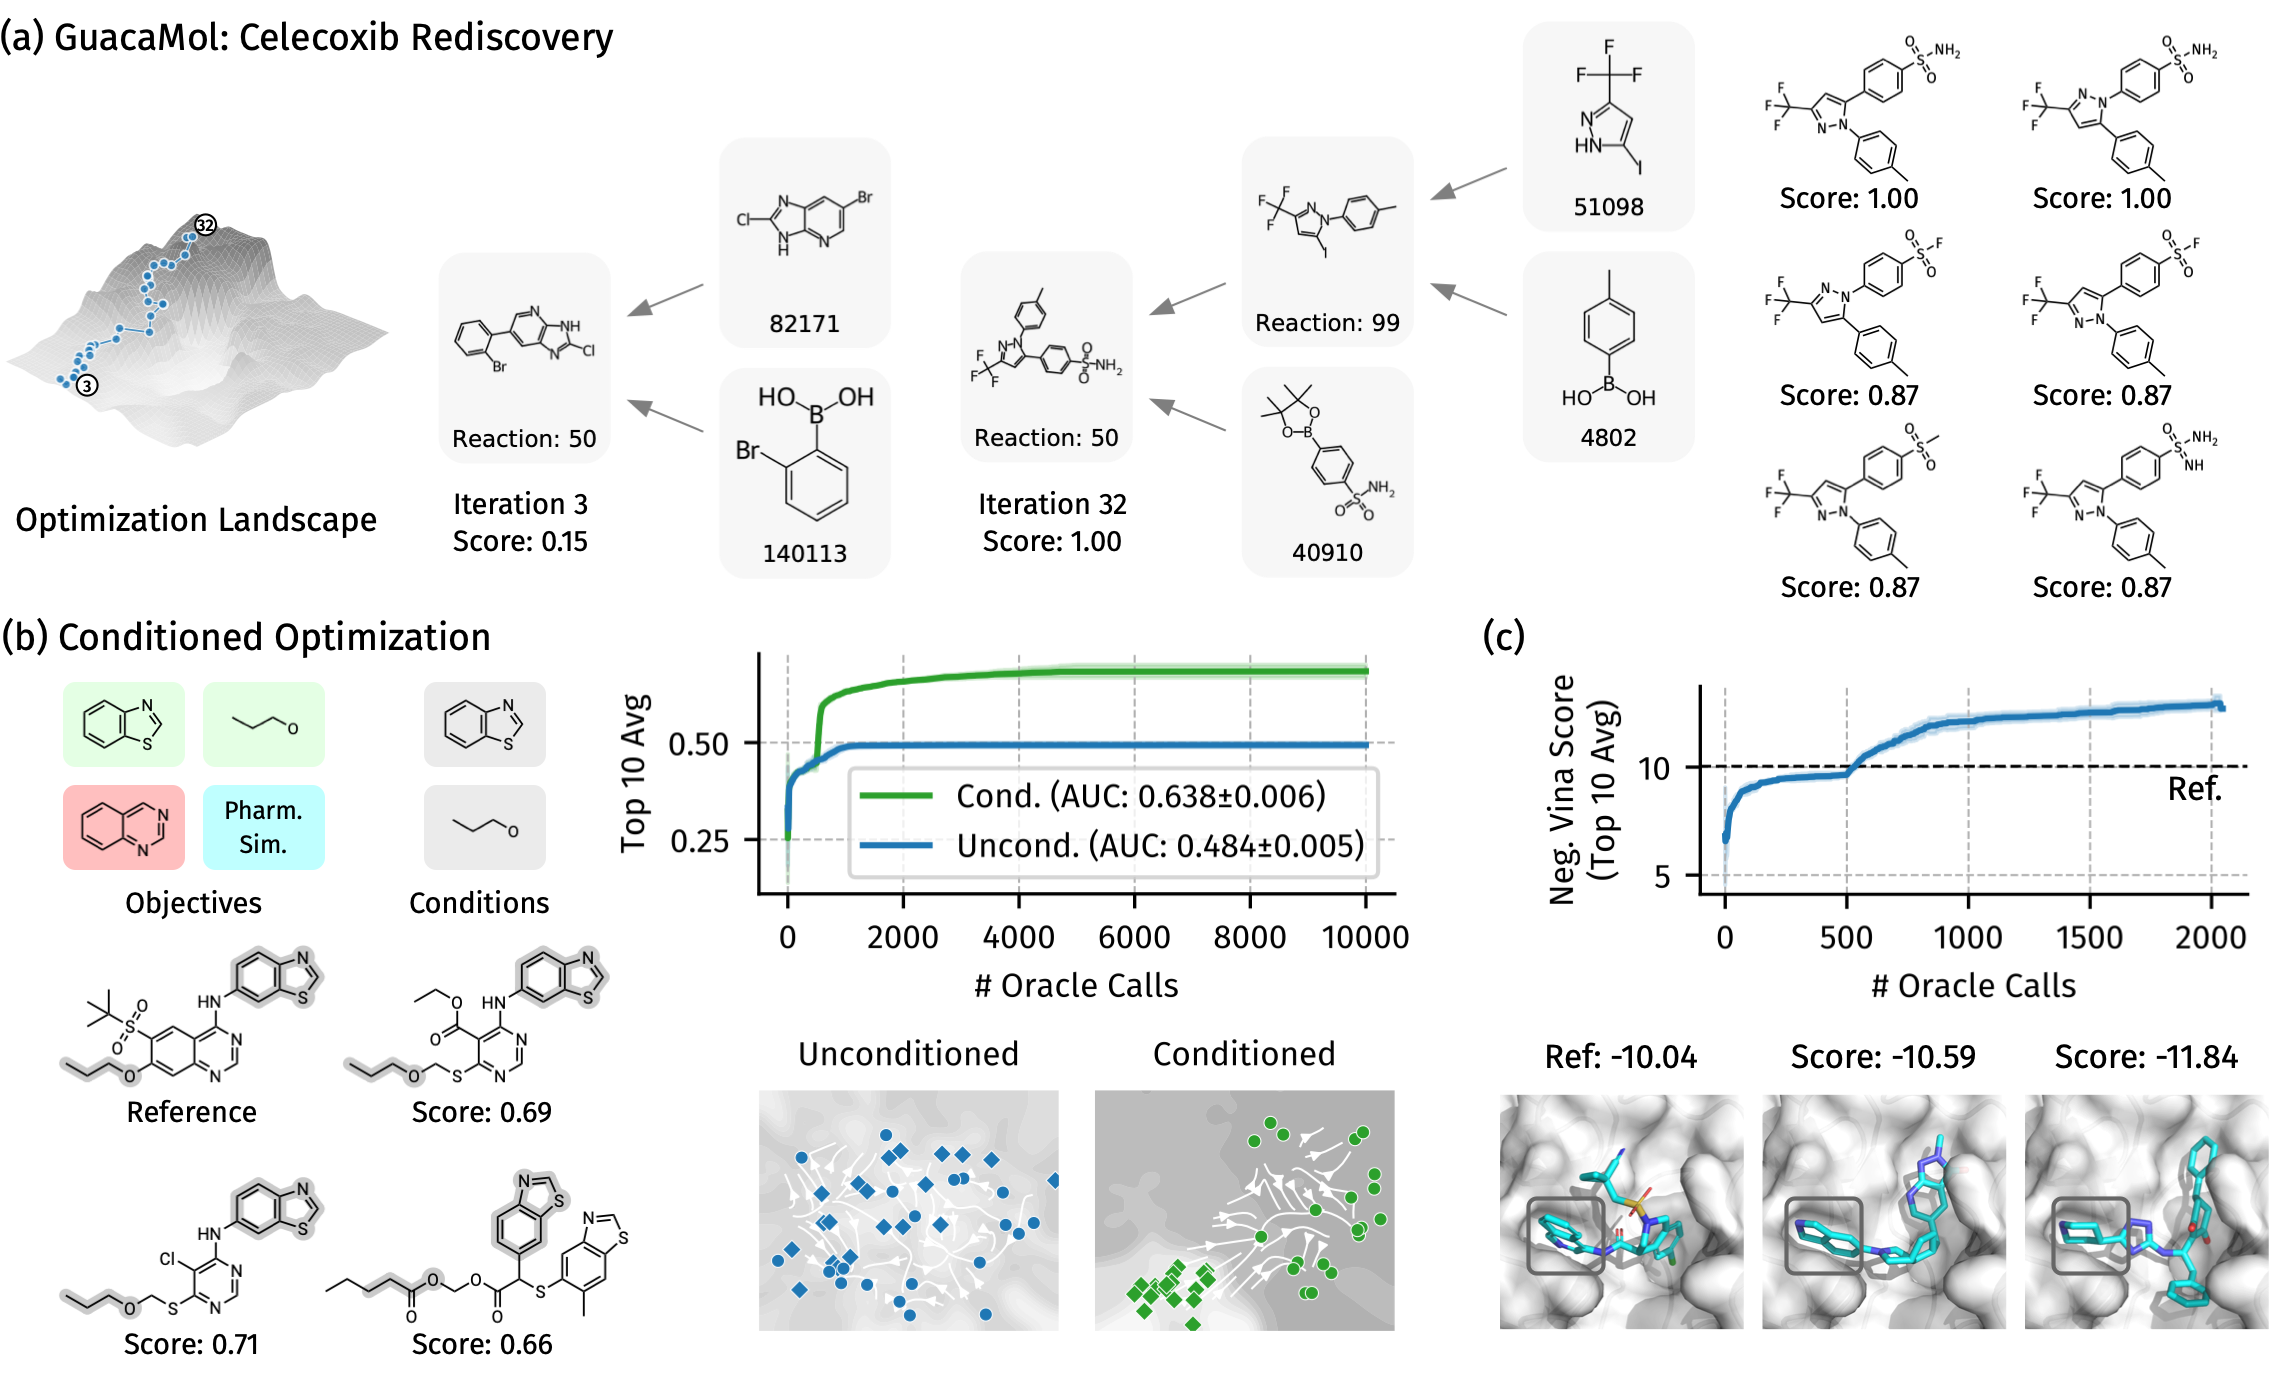
\includegraphics[width=\linewidth]{figures/fig3.png}
  \captionof{figure}{
    \textbf{(a)} Optimization trajectory, two snapshots, and six high-scoring samples for the Celecoxib Rediscovery task. PrexSyn successfully reconstructs Celecoxib and discovers high-scoring analogs.
    \textbf{(b)} Optimization trajectory on the scaffold hopping task with composite property queries. The composite query-conditioned optimization (green curve) achieves higher efficiency than the condition-free baseline (blue curve) and the optimization landscape is smoother.
    \textbf{(c)} Docking score optimization trajectory on the Mpro2 task. PrexSyn generates molecules that achieve improved docking scores compared to the baseline inhibitor (dashed line). The generated molecules share binding modes similar to the baseline inhibitor, including fitting into the highlighted subpocket.
  }
  \label{fig:optimization}
\end{figure}



\begin{table*}[tb]
  \small
  \caption{
    Composite query-based molecular generation results.
    Three tasks reflecting drug discovery scenarios with composite property constraints are designed.
    For each task, we report the mean and standard deviation of both the average score and the diversity of the top 5\% and top 10\% highest-scoring molecules across 5 independent runs. A high score indicates a high degree of compliance to the requested property constraints.
  }
  \label{tab:query}
  \centering
  \begin{adjustbox}{max width=1\textwidth}
  \begin{tabular}{lll cccccc}
\toprule
 & & & Best & \multicolumn{3}{c}{Average Score ($\uparrow$)} & \multicolumn{2}{c}{Diversity ($\uparrow$)}\\
 \# & Task Description & Query & Score & T5\% & T10\% & All & T5\% & T10\% \\
\midrule
1 & \makecell[l]{Generate molecules that \\ satisfy Lipinski's Rule of 5.} & \makecell[l]{\tt MW<500 AND \\ \tt Donors<5 AND \\ \tt Acceptors<10 AND \\ \tt RotatableBonds<10 AND \\ \tt TPSA<140 AND CLogP<5.0} & \makecell{1.0000 \\ $\pm$.0000} & \makecell{1.0000 \\ $\pm$.0000} & \makecell{1.0000 \\ $\pm$.0000} & \makecell{0.9549 \\ $\pm$.0036} & \makecell{0.8902 \\ $\pm$.0011} & \makecell{0.8902 \\ $\pm$.0011}\\
\addlinespace[0.5em]
2 & \makecell[l]{Find analogs of Cobimetinib \\ that have 3 rotatable bonds and \\ 3 aromatic rings. Crippen logP \\ should not exceed 5.0} & \makecell[l]{\tt ECFP4("OC1(CN...") AND \\ \tt RotatableBonds=3 AND \\ \tt AromaticRings=3 AND  \\ \tt CLogP<5.0} & \makecell{0.9326 \\ $\pm$.0040} & \makecell{0.8975 \\ $\pm$.0013} & \makecell{0.8848 \\ $\pm$.0017} & \makecell{0.7108 \\ $\pm$.0060} & \makecell{0.6017 \\ $\pm$.0113} & \makecell{0.6770 \\ $\pm$.0176} \\
\addlinespace[0.5em]
3 & \makecell[l]{Reduce the lipophilicity of \\ Osimertinib by increasing \\ TPSA to above 100 and \\ reducing logP to below 1.0} & \makecell[l]{\tt ECFP4("COc1cc...") AND \\ \tt NOT TPSA<100 AND \\ \tt CLogP<1.0} & \makecell{0.9164 \\ $\pm$.0217} & \makecell{0.8314 \\ $\pm$.0081} & \makecell{0.8068 \\ $\pm$.0047} & \makecell{0.4971 \\ $\pm$.0085} & \makecell{0.7499 \\ $\pm$.0234} & \makecell{0.8024 \\ $\pm$.0061} \\
\bottomrule
\end{tabular}
  \end{adjustbox}
\end{table*}


\subsection{PrexSyn is effective at molecular optimization using docking oracles}

\paragraph{sEH}
We evaluate PrexSyn on the task of generating ligands for soluble epoxide hydrolase (sEH).
The oracle function is defined as the negative docking score predicted by a proxy model trained on molecules docked with AutoDock Vina against the sEH protein structure \citep{cretu2024synflownet,bengio2021flow}.
Following \cite{cretu2024synflownet}, the predicted scores are normalized by a factor of 1/8.

The setting of the baseline method SynFlowNet \citep{cretu2024synflownet} differs from ours. SynFlowNet is trained to learn a distribution of molecules with good docking score, whereas we focus on directly optimizing docking score starting from random molecules. Once trained, SynFlowNet can generate molecules in a single forward pass but requires extensive training data and oracle calls (5000 steps, batch size 64, totaling $\sim$300k samples). In contrast, PrexSyn requires multiple optimization iterations but does not rely on any training samples. While the two settings are not directly comparable, we can still view PrexSyn as a sampler with warm-up steps and compare the quality of generated molecules under a stricter oracle budget. 
Specifically, we allow PrexSyn 10,000 oracle calls, about 30 times fewer than SynFlowNet, and evaluate performance using the top 1,000 generated molecules.

According to Table \ref{tab:seh}, PrexSyn achieves a mean sEH score of 1.01, significantly outperforming SynFlowNet's best-reported score of 0.94.
Note that since the score is defined as the negative binding energy divided by 8, values above 1.0 are possible.
In addition, our generated molecules achieve better drug-likeness, with a QED score of 0.80 compared to SynFlowNet's 0.68, and an improved SA score of 2.23 versus SynFlowNet's 2.67.
While we include the SA score \citep{ertl2009estimation} in the comparison for completeness, we note that SA scores are less relevant in the context of synthesizable molecular design, as providing a synthetic pathway composed only of purchasable building blocks and reaction templates, which both methods do, is a much stronger evidence of synthesizability than the heuristic SA score.

\paragraph{Mpro2}

We further evaluate PrexSyn on the task of generating ligand candidates for the SARS-CoV-2 main protease (Mpro2) using AutoDock-GPU \citep{autodockgpu} as the oracle function.
For this task, we use the protein structure from PDB entry 7GAW, where an inhibitor discovered through the COVID Moonshot project \citep{boby2023open} is co-crystallized with Mpro2. This inhibitor serves as the baseline molecule for evaluation.
We set the initialization query to Lipinski's Rule of 5 to generate drug-like molecules as starting candidates and perform genetic algorithm over the query space containing the ECFP4 fingerprint as the optimizable term.
2,000 oracle calls are budgeted.
As shown in Figure \ref{fig:optimization}c, PrexSyn can generate molecules from scratch that achieve improved docking scores compared to the baseline inhibitor. Visualizations of the docking poses further reveal that the generated molecules share binding modes similar to the baseline inhibitor, including fitting into the highlighted subpocket.


\begin{table}[t]
  \small
  \centering
  \caption{
    sEH docking-based molecular design results.
    PrexSyn outperforms all the baselines in  sEH and QED scores. 
  }
  \label{tab:seh}
  \begin{adjustbox}{max width=1\linewidth}
    \begin{tabular}{l c ccc}
\toprule
Method & Syn. & sEH($\uparrow$) & SA($\downarrow$) & QED($\uparrow$) \\
\midrule
FragGFN \citep{bengio2021flow} & \xmark & 0.77$\pm$0.01 & 6.28$\pm$0.02 & 0.30$\pm$0.01 \\
FragGFN(SA) \citep{bengio2021flow} & \xmark & 0.70$\pm$0.01 & 5.45$\pm$0.05 & 0.29$\pm$0.01 \\
SyntheMol \citep{swanson2024synthemol} & \cmark & 0.64$\pm$0.01 & 3.08$\pm$0.01 & 0.63$\pm$0.01 \\
SynFlowNet \citep{cretu2024synflownet} & \cmark & 0.92$\pm$0.01 & 2.92$\pm$0.01 & 0.59$\pm$0.02 \\
SynFlowNet(SA) \citep{cretu2024synflownet} & \cmark & 0.94$\pm$0.01 & 2.67$\pm$0.03 & 0.68$\pm$0.01 \\
SynFlowNet(QED) \citep{cretu2024synflownet} & \cmark & 0.86$\pm$0.03 & 4.02$\pm$0.26 & 0.74$\pm$0.04 \\
ReaSyn \citep{lee2025rethinking} & \cmark & 0.97$\pm$0.01 & \bf 2.01$\pm$0.02 & 0.75$\pm$0.01 \\
\midrule
PrexSyn  & \cmark & \bf 1.01$\pm$0.00 & 2.23$\pm$0.04 & \bf 0.80$\pm$0.01 \\
\bottomrule
\end{tabular}
  \end{adjustbox}
\end{table}
